
% 3. Environnement unique et superposition directe
\begin{tikzpicture}
  % On dessine les deux éléments sur le MÊME repère absolu
  \clip[](-1.3, -1.2) rectangle (1.5 , 1.1)  ;

  \node[transform canvas={scale=1}] at (0,0) {
    \begin{tikzpicture}

        \begin{scope}[shift={(-0.0,0.0)}, xscale=1,yscale=1]
            % Grille principale
            \draw[opacity=0.2,very thin,line width=0.01cm,color=colorThree](-0.15,-0.15)grid(1.95,1.95);
            % Sous-grille
            \draw[opacity=0.2,very thin,line width=0.01cm,color=colorThree](-0.15,-0.15)grid[step=0.1](2.35,1.95);

            % Graduations X
            \foreach \x in {-0.1,0,0.1,...,2.4} {
                \draw[line width=0.01cm,color=colorOne](\x,0-0.03)--(\x,0+0.03);
            }
            \foreach \x in {1,...,2} {
                \draw[line width=0.01cm,color=colorOne](\x,0-0.05)--(\x,0+0.05)
                node[shift={(0,0.05)},font=\fontsize{0.05cm}{0.05cm}\bfseries\selectfont]{\x};
            }
            % Graduations Y
             \foreach \y in {-0.1,0,0.1,...,2} {
                \draw[line width=0.01cm,color=colorOne,](0-0.03,\y)--(0+0.03,\y);
            }
            \foreach \y in {1,...,1} {
                \draw[line width=0.01cm,color=colorOne,](0-0.05,\y)--(0+0.05,\y)
                node[shift={(-0.15,0)},font=\fontsize{0.05cm}{0.05cm}\bfseries\selectfont]{\y};
            }

            % 2. Axe des abscisses (x)
            \draw[line width=0.01cm,color=colorOne,->,
            >={Computer Modern Rightarrow[length=0.04cm, width=0.06cm]}
            ] (-0.15,0) -- (2.4,0) 
                node[pos=1.0, xshift=-0.06cm,yshift=-0.05cm, color=colorOne, font=\fontsize{0.05cm}{0.05cm}\bfseries\selectfont] {$x$};

            % 3. Axe des ordonnées (S(x))
            \draw[line width=0.01cm,color=colorOne,->,
            >={Computer Modern Rightarrow[length=0.04cm, width=0.06cm]}
            ] (0,-0.15) -- (0,2) 
                node[pos=1.0, xshift=-0.05cm,yshift=-0.06cm, color=colorOne, font=\fontsize{0.05cm}{0.05cm}\bfseries\selectfont] {$y$}
                ;

        \end{scope}
        
        

        % 4. Courbe de la parabole y = x^2 (domaine restreint pour rester dans le cadre)
        %\draw[smooth, line width=1.0ex, color=colorFour, domain=-2.1:2.1, samples=100] plot (\x, {1-2*\x*\x});

        \def\xzeroA{0.2} \def\yzeroA{0.2} \def\xzeroB{2}  \def\yzeroB{1.9} \def\vzeroscale{2}  \def\g{9.81} \def\dt{0.05} 

        \def\listeLabels{
            0//M_0///,
            1/////,
            2////,
            3//M_3///,
            4//M_4///,
            5//M_5///,
            6//M_6///,
            7//M_7///,
            8//M_8///,
            9//M_9///,
            10//M_{10}///,
            11//M_{11}///,
            12//M_{12}///,
        }

        \foreach \n/\labelBottom/\labelTop/\LabelvecPos/\LabelvecVit/\LabelvecAcc in \listeLabels {%

            \pgfmathsetmacro{\t}{\n*\dt}
            \pgfmathsetmacro{\xA}{\xzeroA + (\xzeroB-\xzeroA)*\vzeroscale*\t}
            \pgfmathsetmacro{\yA}{\yzeroA + (\yzeroB-\yzeroA)*\vzeroscale*\t - 0.5*\g*\t*\t}
            \pgfmathsetmacro{\xB}{\xzeroB}
            \pgfmathsetmacro{\yB}{\yzeroB - 0.5*\g*\t*\t}

            % Point
            \fill[opacity = 0.5, color=colorFour] (\xA,\yA) circle (0.01);
            \fill[opacity = 0.5, color=colorSix] (\xB,\yB) circle (0.01);

            % Label inférieur
            \if\relax\detokenize{\labelBottom}\relax
            \else
                \node[below,font=\fontsize{0.05cm}{0.05cm}\bfseries\selectfont] at (\xA,\yA) {$\labelBottom$};
                \node[below,font=\fontsize{0.05cm}{0.05cm}\bfseries\selectfont] at (\xB,\yB) {$\labelBottom$};
            \fi

            % Label supérieur
            \if\relax\detokenize{\labelTop}\relax
            \else
                \node[font=\fontsize{0.05cm}{0.05cm}\bfseries\selectfont] at (\xA+0.05,\yA+0.05) {$\labelTop$};
                \node[font=\fontsize{0.05cm}{0.05cm}\bfseries\selectfont] at (\xB+0.05,\yB+0.05) {$\labelTop$};
            \fi

            
        }
        

        \pgfmathsetmacro{\xvec}{\xzeroA+(\xzeroB-\xzeroA)*\vzeroscale/10}
        \pgfmathsetmacro{\yvec}{\yzeroA+(\yzeroB-\yzeroA)*\vzeroscale/10}

        \draw[opacity = 1,line width=0.01cm,shift={(0,0)}]
            (\xzeroA,\yzeroA)edge[shift={(0,0)}, opacity = 0.5 , dashed, color=colorThree]node[pos=0.5,shift={(0.02cm,0.1cm)},color=colorOne,font=\fontsize{0.1cm}{0.04cm}\bfseries\selectfont, rotate = 0]{$ $}(\xzeroB,\yzeroB)
            (\xzeroA,\yzeroA)edge[shift={(0,0)},color=colorOne,-{Computer Modern Rightarrow[length=0.04cm,width=0.06cm]}]node[pos=0.5,shift={(0.02cm,0.1cm)},color=colorOne,font=\fontsize{0.1cm}{0.04cm}\bfseries\selectfont, rotate = 0]{$ \vec{v}_0$}(\xvec,\yvec)
            (1.7,1.9)edge[shift={(0,0)},color=colorSix,-{Computer Modern Rightarrow[length=0.04cm,width=0.06cm]}]node[pos=0.5,shift={(0.05cm,0.03cm)},color=colorSix,font=\fontsize{0.05cm}{0.04cm}\bfseries\selectfont, rotate = -90]{$ \vec{g} = - g\vec{u}_x $}(1.7,1.9-\g/20)
        ;


        %vague
        \draw [decoration={snake, amplitude=0.02cm, segment length=0.2cm},]
            (0,0.2) edge[ decorate, color=colorFour , line width=0.01cm,] (2,0.2)
        ;

        %poisson
        \node[transform canvas={scale=0.2}] at (1,1) {

            \begin{tikzpicture}[]

                % --- JET D'EAU ---
                \draw[cyan!60!blue, line width=1.5pt, line cap=round, dash pattern=on 10pt off 3pt on 3pt off 3pt] 
                    (2.8, 0.4) .. controls (3.5, 1.2) and (4.5, 2.5) .. (5, 4);
                \fill[cyan!60!blue] (5, 4.1) circle (1.5pt); % Goutte supérieure
                \fill[cyan!60!blue] (4.8, 3.7) circle (1pt);

                % --- CORPS DU POISSON ---
                % Dos et ventre (forme générale fuselée)
                \draw[thick, fill=yellow!25!gray!20] 
                    (0,0) .. controls (1, 1.2) and (2.5, 1) .. (3, 0.3) % Dos
                    .. controls (2.5, -0.8) and (1, -0.8) .. (0,0); % Ventre

                % --- BANDES NOIRES (Caractéristique du poisson-archer) ---
                \begin{scope}
                    % On clip pour que les bandes restent dans le corps du poisson
                    \clip (0,0) .. controls (1, 1.2) and (2.5, 1) .. (3, 0.3) .. controls (2.5, -0.8) and (1, -0.8) .. (0,0);
                    \fill[black!85] (0.8, 1) -- (1.2, 1) -- (1.0, -0.5) -- (0.7, -0.5) -- cycle;
                    \fill[black!85] (1.5, 1) -- (1.9, 1) -- (1.6, -0.6) -- (1.3, -0.6) -- cycle;
                    \fill[black!85] (2.2, 0.9) -- (2.5, 0.8) -- (2.2, -0.4) -- (2.0, -0.4) -- cycle;
                \end{scope}

                % --- NAGEOIRES ---
                % Nageoire caudale (Queue)
                \draw[thick, fill=yellow!60!black!30] 
                    (0,0) -- (-0.6, 0.4) -- (-0.5, 0) -- (-0.6, -0.4) -- cycle;
                
                % Nageoire dorsale (Reculée sur le dos)
                \draw[thick, fill=yellow!60!black!40] 
                    (2.0, 0.65) .. controls (2.3, 1.1) .. (2.6, 0.9) -- (2.5, 0.45) -- cycle;
                    
                % Nageoire anale
                \draw[thick, fill=yellow!60!black!40] 
                    (1.8, -0.55) .. controls (2.1, -0.9) .. (2.5, -0.6) -- (2.4, -0.3) -- cycle;

                % Nageoire pectorale
                \draw[thick, fill=yellow!50!white!50, opacity=0.8] 
                    (1.1, -0.1) .. controls (1.4, -0.1) and (1.5, -0.4) .. (1.3, -0.5) .. controls (1.1, -0.4) .. (1.1, -0.1);

                % --- TÊTE ET BOUCHE ---
                % Œil (Grand et bas, typique)
                \fill[black] (2.4, 0.25) circle (2.5pt);
                \draw[black, thin] (2.4, 0.25) circle (4pt);
                
                % Bouche pointée vers le haut (prête à tirer)
                \draw[thick, line cap=round] (2.9, 0.15) -- (3.1, 0.3) -- (2.8, 0.35);
                \draw[thin] (2.95, 0.25) -- (3.05, 0.28); % Ligne de la bouche

                % Ouïes
                \draw[black!60, thin] (2.0, 0.2) .. controls (1.9, 0.0) and (1.9, -0.2) .. (2.1, -0.4);

            \end{tikzpicture}

        }
        
        %mouche
        \node[transform canvas={scale=0.2}] at (3,3) {
            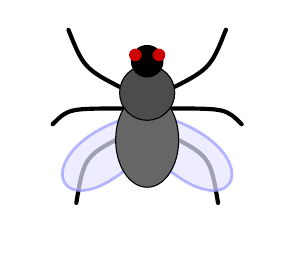
\begin{tikzpicture}[scale=1]

                % Pattes gauches
                \draw [line width=1.5pt, line cap=round] (-0.2,0.2) .. controls (-0.8,0.5) .. (-1,1);
                \draw [line width=1.5pt, line cap=round] (-0.3,0) .. controls (-1,0) .. (-1.2,-0.2);
                \draw [line width=1.5pt, line cap=round] (-0.2,-0.3) .. controls (-0.8,-0.6) .. (-0.9,-1.2);

                % Pattes droites
                \draw [line width=1.5pt, line cap=round] (0.2,0.2) .. controls (0.8,0.5) .. (1,1);
                \draw [line width=1.5pt, line cap=round] (0.3,0) .. controls (1,0) .. (1.2,-0.2);
                \draw [line width=1.5pt, line cap=round] (0.2,-0.3) .. controls (0.8,-0.6) .. (0.9,-1.2);

                % Aile gauche (transparente)
                \filldraw [fill=blue!10, draw=blue!40, opacity=0.7, line width=1pt] 
                    (-0.2,-0.1) .. controls (-1.5,-0.5) and (-1.2,-1.5) .. (-0.3,-0.8) -- cycle;

                % Aile droite (transparente)
                \filldraw [fill=blue!10, draw=blue!40, opacity=0.7, line width=1pt] 
                    (0.2,-0.1) .. controls (1.5,-0.5) and (1.2,-1.5) .. (0.3,-0.8) -- cycle;

                % Corps (Abdomen)
                \filldraw [fill=gray!80!black, draw=black] (0,-0.4) ellipse (0.4cm and 0.6cm);

                % Thorax
                \filldraw [fill=gray!60!black, draw=black] (0,0.2) circle (0.35cm);

                % Tête
                \filldraw [fill=black] (0,0.6) circle (0.2cm);

                % Yeux (rouges)
                \fill [red!80!black] (-0.15,0.68) circle (0.08cm);
                \fill [red!80!black] (0.15,0.68) circle (0.08cm);

            \end{tikzpicture}

        }


        

     \end{tikzpicture}
};
        

  % Grille de repérage
  %\draw[line width=0.5ex , color = red] (-1.3, -1.2) rectangle (1.5 , 1.1) ;
  %\drawgrid{-6.1}{6.2}{-5.5}{4.5}{1}{1}
\end{tikzpicture}



